\documentclass[12pt]{article}
\usepackage[letterpaper,margin=1in]{geometry}
\usepackage{setspace}
\usepackage{amsmath}
\usepackage{booktabs}
\usepackage{graphicx}
\usepackage{float}
\usepackage[hyphens]{url}
\usepackage{multicol}
\doublespacing
\setlength{\parskip}{0pt}
\urlstyle{same}
\setlength{\intextsep}{6pt plus 2pt minus 2pt}
\setlength{\abovecaptionskip}{3pt}
\setlength{\belowcaptionskip}{0pt}
\begin{document}

\title{A Knowledge-Based AI Framework for Data-Driven Cost-Aware Classification: Decision Support for Digital Transformation in Entrepreneurial Credit Innovation}
\author{%
Pravallika Nalluri\textsuperscript{a}\\[0.4em]
\normalsize \textsuperscript{a}Independent Researcher, USA\\[0.25em]
\normalsize Corresponding author. Email: pravallikanalluri9848@gmail.com%
}
\date{}
\maketitle

\begin{abstract}
\noindent
Credit decisions need an explicit cost for a missed default, not only a probability. This study states a normalized decision cost and compares two knowledge-based rules that turn probabilities into a yes-or-no action. Both rules are locked on a validation split before the test evaluation. On the UCI credit-card default file (30,000 accounts; 6,636 defaults, 22.12\%), four probability models were fit without class weights. On the primary split (seed 42), prediction-first selection kept histogram gradient boosting, the model with the highest validation F1 at threshold 0.50 (0.4682), and then chose a cost-minimizing threshold. Decision-first selection searched every model and threshold for the lowest validation cost. Decision-first selection had the lower test cost at a false-negative cost ratio of 2 (relative difference 0.0406; paired bootstrap 95\% interval for the cost difference, 0.0050 to 0.0210). At ratios 5, 10, and 20 that interval included zero, so the strategy difference is not statistically conclusive. Leaving threshold 0.50 reduced test cost at ratios 5, 10, and 20, and those intervals excluded zero; at ratio 2 the threshold contrast was not statistically conclusive. On 20 stratified splits (seeds 42 through 61), tuned test cost was lower than the cost at 0.50 on 19 of 20 splits at ratio 2 and on all 20 splits at ratios 5, 10, and 20. Ranges across splits are not confidence intervals. The public file is not a startup portfolio.
\end{abstract}

{\sloppy\noindent\textbf{Keywords:} Cost-sensitive classification; Decision support; Decision threshold; Knowledge-based system; Credit scoring; Digital transformation\par}

\section{Introduction}
Knowledge-based systems support a human decision, not only a ranked score. In credit, a probability of default is not itself an action. Decision-support credit scoring and automatic threshold learning already treat that action as the object to be chosen \cite{idbenjra2024,li2024}, and misclassification costs can be turned into explicit rules and trees \cite{kopanja2025}. This short communication keeps a simpler piece of knowledge. A lender writes down one false-negative cost ratio before any test account is scored, and that ratio selects a threshold another person can inspect.

\begin{singlespace}\small
Cost-sensitive objectives are used for default prediction, reject inference, credit-risk learning, company financial-distress prediction, and asymmetric-loss assessment \cite{xing2024,shen2024,crella2025,wangchi2024,zhao2024}. Some of those costs vary by account \cite{xing2024,crella2025}. Profit-driven scoring replaces a single ratio with a monetary loss \cite{xukou2025,xuergu2026}. The ratio \(r\) in this study is a scenario weight, not an estimated loss and not a per-account cost. Imbalance is often carried by the learner, by a changed boosting loss, or by resampling and augmentation \cite{tang2024,mushava2024,weng2025,nazri2025,sun2024,ranjan2024}. None of those devices is used here. Four probability models are fit without class weights, and the threshold grid carries both the base rate and \(r\).

Predictive comparisons are already a large literature: imbalanced and interpretable scoring \cite{chen2024,tu2025}, ensembles \cite{kwon2025,yang2024}, credit-card customer models \cite{chang2024}, stacking that brings in business knowledge \cite{ding2025}, cross-institution imbalanced scoring \cite{wang2025ejor}, and XGBoost hyperparameter search \cite{vikas2025}. This short communication does not add another accuracy contest.
\end{singlespace}
\doublespacing Prediction-first selection fixes the model by validation F1 at threshold 0.50, then tunes only the threshold. Decision-first selection chooses the model and the threshold together by validation cost. On each split, the test set is scored once, after both rules are locked. The contribution is Eq.~\eqref{eq:cost}, the two selection rules in Eqs.~\eqref{eq:strategy-a} and \eqref{eq:strategy-b}, and the same lock repeated on 20 stratified splits. Section~\ref{sec:results} separates the gap between the rules from the move away from threshold 0.50. The study does not claim that decision-first selection is uniformly superior. The comparison uses the public Default of Credit Card Clients file \cite{yeh2009,yehdata}.

\section{Decision framework}
\label{sec:framework}
The positive class is default payment next month. A model emits a probability, and the decision predicts default when that probability is at least a threshold \(t\). A false positive is a predicted default that does not occur. A false negative is a missed default. With \(N\) cases in the split being scored, the normalized cost per case at false-negative ratio \(r\) is
\begin{equation}
c(r)=\frac{1\cdot\mathrm{FP}+r\cdot\mathrm{FN}}{N}.
\label{eq:cost}
\end{equation}
The ratio \(r\) is a scenario weight, not an estimated monetary loss. The values used here are \(r\in\{2,5,10,20\}\). The threshold grid is \(\mathcal{T}=\{0.01,0.02,\ldots,0.99\}\).

Let \(m\) index the candidate models, and let \(\mathrm{F1}_{\mathrm{val}}\) be the positive-class F1 on the validation split. Prediction-first selection fixes one model, then one threshold for each \(r\):
\begin{equation}
\begin{aligned}
m^{*}&=\arg\max_{m}\mathrm{F1}_{\mathrm{val}}(m,0.50),\\
t_{A}^{*}(r)&=\arg\min_{t\in\mathcal{T}}c_{\mathrm{val}}(m^{*},t,r).
\end{aligned}
\label{eq:strategy-a}
\end{equation}
If several models share the highest validation F1 at 0.50, the tie is broken by the lower validation cost at that same threshold for the \(r\) under consideration, then by model name in alphabetical order. The threshold tie is broken by higher validation F1, then by the lower threshold.

Decision-first selection searches the pairs directly:
\begin{equation}
\bigl(m_{B}^{*}(r),t_{B}^{*}(r)\bigr)
=\arg\min_{m,\,t\in\mathcal{T}}c_{\mathrm{val}}(m,t,r).
\label{eq:strategy-b}
\end{equation}
Ties are broken by higher validation F1 at that threshold, then by model name, then by the lower threshold. Class imbalance is not handled with class weights. The grid search is the mechanism that carries both the base rate and the cost ratio. Neither rule may use the test split.

\section{Experimental design}
The source file is the UCI Default of Credit Card Clients workbook \cite{yeh2009,yehdata}. It has 30,000 accounts and 6,636 defaults (22.12\%). The same file is still used for predictive comparisons \cite{bhandary2025}. The identifier column is dropped. The public file contains SEX. Algorithmic bias in credit scoring support systems is an active design problem \cite{lin2026}. SEX is removed before the split because a credit decision policy should not use sex, and this study does not estimate a sex effect. The other 22 predictors are kept as the numeric codes in the file, including education, marriage, age, recent repayment status, bill amounts, and payment amounts.

The split and the bootstrap each use seed 42. The split is stratified. It holds out 6,000 test accounts and then holds out 6,000 validation accounts, leaving 18,000 training accounts. Models are fit only on the training accounts. Selection uses only the validation accounts. Test probabilities are computed after every model and threshold has been chosen.

Four models produce probabilities, with random seed 42 wherever the implementation accepts one, and with no class weight. A logistic regression uses $C = 1$, after a standardizer, with the library's default L2 penalty. The other models are a random forest (200 trees, depth 10, minimum leaf size 5), histogram gradient boosting (200 iterations, depth 6, learning rate 0.1), and XGBoost (200 trees, depth 5, learning rate 0.1). Thresholds run from 0.01 to 0.99 in steps of 0.01. The decision predicts default when the probability is at least the threshold.

Uncertainty is a paired bootstrap of the test accounts: 1,000 resamples, percentile interval from 2.5 to 97.5, seed 42. The same resamples are used for every contrast. The procedure does not refit models and does not rerun selection. A positive strategy difference means decision-first selection has the lower test cost. The relative difference is that gap divided by the prediction-first test cost. If an interval includes zero, the difference is not statistically conclusive. Seeds 42 through 61 repeat the same stratified sizes, 20 splits in total, with the model random seed held at 42. The minimum, median, and maximum across those splits are a stability range. They are not a confidence interval.

\section{Results}
\label{sec:results}
Table~\ref{tab:validation} is the validation lock. Validation F1 at threshold 0.50 selected histogram gradient boosting. Its F1 was higher than that of the random forest, XGBoost, and logistic regression, and the four values were distinct, so the cost tie-break was not used. On this split the prediction-first model is therefore fixed for every cost ratio. As \(r\) increases, the chosen threshold falls. For histogram gradient boosting the validation thresholds are 0.31, 0.16, 0.09, and 0.01. The last of these is the bottom of the grid, so the search could not move lower. That edge is also selected on 6 of the 20 splits. Decision-first selection chooses the random forest at \(r=2\), \(r=10\), and \(r=20\), and XGBoost at \(r=5\).

\begin{table}[htbp]
\centering
\begin{singlespace}
\caption{Validation choice for each false-negative cost ratio. Cost is Eq.~\eqref{eq:cost} on the validation split. F1 is the positive-class F1 at the chosen threshold.}
\label{tab:validation}
\footnotesize
\begin{tabular}{@{}r l l c c c@{}}
\toprule
\(r\) & Strategy & Model & Threshold & Val.\ cost & Val.\ F1 \\
\midrule
2 & A & histogram GB & 0.31 & 0.3075 & 0.5343 \\
2 & B & random forest & 0.30 & 0.2975 & 0.5502 \\
5 & A & histogram GB & 0.16 & 0.5485 & 0.5050 \\
5 & B & XGBoost & 0.16 & 0.5318 & 0.5126 \\
10 & A & histogram GB & 0.09 & 0.7065 & 0.4414 \\
10 & B & random forest & 0.10 & 0.6982 & 0.4259 \\
20 & A & histogram GB & 0.01 & 0.7728 & 0.3656 \\
20 & B & random forest & 0.06 & 0.7645 & 0.3738 \\
\bottomrule
\end{tabular}
\par\vspace{0.35em}
\parbox{\linewidth}{\footnotesize Strategy A uses one model for every \(r\), selected by validation F1 at threshold 0.50: logistic regression 0.3694; random forest 0.4658; histogram GB 0.4682; XGBoost 0.4598. The F1 values were distinct, so the cost tie-break was not used. Strategy B minimizes validation cost over models and thresholds. Histogram GB denotes histogram gradient boosting.}
\end{singlespace}
\end{table}

On the locked test split, the strategy gap is small relative to the cost of staying at threshold 0.50 (Table~\ref{tab:test} and Figure~\ref{fig:costs}). At \(r=2\), decision-first selection reaches test cost 0.3035 and prediction-first selection reaches 0.3163. The relative difference is 0.0406. The 95\% interval for the cost difference is 0.0050 to 0.0210 and excludes zero, so this difference is statistically conclusive on the present test set. At \(r=5\), the prediction-first cost is slightly lower (0.5762 versus 0.5788; relative difference \(-0.0046\)). The interval includes zero, and the difference is not statistically conclusive. At \(r=10\) and \(r=20\) the point estimates favor decision-first selection (relative differences 0.0401 and 0.0077), but both intervals include zero. Those differences are not statistically conclusive. Decision-first selection is therefore not uniformly cheaper on this file.

\begin{table}[htbp]
\centering
\begin{singlespace}
\caption{Test cost per case after selection was locked. A positive value of \((A-B)/A\) means strategy B has the lower test cost. The 95\% interval is a paired percentile bootstrap of the test-cost difference \(A-B\). It does not refit the models.}
\label{tab:test}
\footnotesize
\begin{tabular}{@{}r l l c c@{}}
\toprule
\(r\) & Strategy & Model & Threshold & Test cost \\
\midrule
2 & A & histogram GB & 0.31 & 0.3163 \\
2 & B & random forest & 0.30 & 0.3035 \\
\multicolumn{5}{@{}p{\linewidth}@{}}{\footnotesize $(A-B)/A = 0.0406$. Cost difference $A-B = 0.0128$, 95\% CI $[0.0050,\ 0.0210]$, includes zero: no.} \\
\addlinespace
5 & A & histogram GB & 0.16 & 0.5762 \\
5 & B & XGBoost & 0.16 & 0.5788 \\
\multicolumn{5}{@{}p{\linewidth}@{}}{\footnotesize $(A-B)/A = -0.0046$. Cost difference $A-B = -0.0027$, 95\% CI $[-0.0202,\ 0.0147]$, includes zero: yes.} \\
\addlinespace
10 & A & histogram GB & 0.09 & 0.7392 \\
10 & B & random forest & 0.10 & 0.7095 \\
\multicolumn{5}{@{}p{\linewidth}@{}}{\footnotesize $(A-B)/A = 0.0401$. Cost difference $A-B = 0.0297$, 95\% CI $[-0.0023,\ 0.0655]$, includes zero: yes.} \\
\addlinespace
20 & A & histogram GB & 0.01 & 0.7815 \\
20 & B & random forest & 0.06 & 0.7755 \\
\multicolumn{5}{@{}p{\linewidth}@{}}{\footnotesize $(A-B)/A = 0.0077$. Cost difference $A-B = 0.0060$, 95\% CI $[-0.0168,\ 0.0272]$, includes zero: yes.} \\
\bottomrule
\end{tabular}
\par\vspace{0.35em}
\parbox{\linewidth}{\footnotesize For the prediction-first model (histogram GB), test cost at threshold 0.50 versus the cost-tuned threshold: $r=2$, 0.3272 versus 0.3163; $r=5$, 0.7522 versus 0.5762; $r=10$, 1.4605 versus 0.7392; $r=20$, 2.8772 versus 0.7815. Paired bootstrap 95\% CIs for (cost at 0.50 minus cost at the tuned threshold) are $r=2$, $[-0.0008,\ 0.0227]$, includes zero: yes; $r=5$, $[0.1370,\ 0.2147]$, includes zero: no; $r=10$, $[0.6297,\ 0.8035]$, includes zero: no; $r=20$, $[1.9144,\ 2.2858]$, includes zero: no. Across seeds 42 through 61 (20 splits), prediction-first test cost min, median, and max were $r=2$, 0.2917, 0.3052, 0.3175; $r=5$, 0.5253, 0.5617, 0.5762; $r=10$, 0.6668, 0.7163, 0.7472; $r=20$, 0.7673, 0.7792, 0.8660. Cost at threshold 0.50 min, median, and max were $r=2$, 0.3122, 0.3196, 0.3300; $r=5$, 0.7212, 0.7372, 0.7655; $r=10$, 1.4002, 1.4343, 1.4913; $r=20$, 2.7552, 2.8276, 2.9430. Decision-first test cost min, median, and max were $r=2$, 0.2930, 0.3035, 0.3143; $r=5$, 0.5435, 0.5581, 0.5880; $r=10$, 0.6625, 0.7038, 0.7457; $r=20$, 0.7523, 0.7654, 0.7965. Tuned cost was lower on 19 of 20 splits at $r=2$ and on 20 of 20 splits at $r=5$, $r=10$, and $r=20$. Decision-first test cost was strictly lower on 13, 7, 13, and 17 of 20 splits. These ranges are not a confidence interval.}
\end{singlespace}
\end{table}

The larger change is the threshold, not the selector. At \(r=2\), test cost moves from 0.3272 at threshold 0.50 to 0.3163, and that interval includes zero. At \(r=5\), \(r=10\), and \(r=20\), the contrast falls from 0.7522 to 0.5762, from 1.4605 to 0.7392, and from 2.8772 to 0.7815, and those intervals exclude zero. Figure~\ref{fig:curves} is the validation curve for the seed-42 thresholds. Across seeds 42 through 61, the prediction-first model was histogram gradient boosting on 12 splits, XGBoost on 6, and the random forest on 2. No split used the cost tie-break. Prediction-first thresholds ranged from 0.30 to 0.38 at \(r=2\), 0.13 to 0.22 at \(r=5\), 0.05 to 0.10 at \(r=10\), and 0.01 to 0.08 at \(r=20\). Decision-first selection chose the random forest on 18, 12, 17, and 18 of the 20 splits. The whiskers in Figure~\ref{fig:costs} are those minima and maxima. They are not a confidence interval.

\begin{figure}[H]
\centering
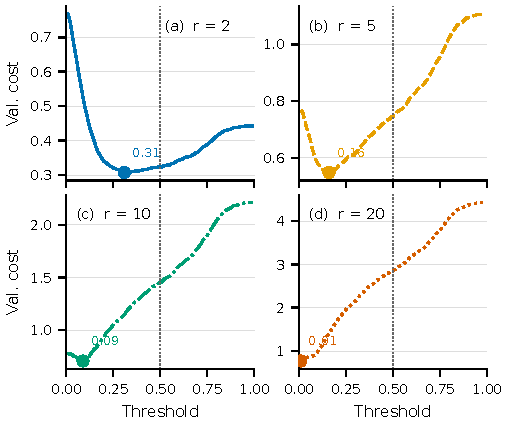
\includegraphics[width=7.6cm]{Figure_1.pdf}
\begin{singlespace}
\caption{Validation cost per case for the prediction-first model on the seed-42 validation split. Panels (a)--(d) are the cost ratios 2, 5, 10, and 20. The curve is Eq.~\eqref{eq:cost}. The circle marks the minimizing threshold and is labeled with its value. The dotted line is threshold 0.50.}
\label{fig:curves}
\end{singlespace}
\end{figure}

\begin{figure}[H]
\centering
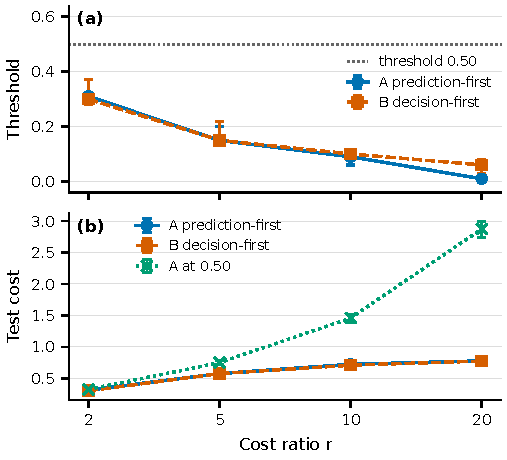
\includegraphics[width=7.6cm]{Figure_2.pdf}
\begin{singlespace}
\caption{Chosen threshold (a) and test cost per case (b) across false-negative cost ratios. Markers are the seed-42 rules. Circles are prediction-first selection. Squares are decision-first selection. Crosses score the prediction-first model at threshold 0.50. Whiskers run from the minimum to the maximum over 20 stratified splits (seeds 42 through 61). They are not a confidence interval. The dotted line in (a) is threshold 0.50. Model names for seed 42 are in Table~\ref{tab:test}.}
\label{fig:costs}
\end{singlespace}
\end{figure}

\section{Implications for entrepreneurial credit decisions}
A credit operation, including a smaller lending venture, writes down \(r\) and publishes the threshold from Eq.~\eqref{eq:strategy-a} or Eq.~\eqref{eq:strategy-b}. On this file, \(r=10\) moves the prediction-first rule from 0.50 to 0.09. Online consumer credit is already framed as a risk-management task \cite{zhu2024}. Digital-transformation research treats the organizational resource, rather than the software alone, as what has to change \cite{piccoli2024}. Here that resource is the pair \((r,t)\). The UCI file contains Taiwanese credit-card clients \cite{yeh2009}. It is not a startup portfolio, and \(r\) is a scenario weight rather than a measured loss.

\section{Conclusion}
The useful output is a threshold tied to a stated cost ratio. Decision-first selection was conclusively cheaper only at \(r=2\). At \(r=5\), \(r=10\), and \(r=20\), the strategy difference was not statistically conclusive. Across seeds 42 through 61, tuned test cost was lower than the cost at 0.50 on all 20 splits at the three higher ratios, and that range is not a confidence interval. The \(r=20\) prediction-first threshold sits on the lower edge of the grid. SEX was excluded from the predictors and was not used to estimate a sex effect.

\begin{singlespace}
\section*{Data availability}
The Default of Credit Card Clients file is the UCI Machine Learning Repository dataset introduced by Yeh and Lien \cite{yeh2009,yehdata} (\url{https://doi.org/10.24432/C55S3H}). The script that regenerates the tables and figures is \texttt{run.py} in \url{https://github.com/pravallika-nalluri-dba/kbs-cost-aware-classification}.

\section*{Declaration of competing interest}
The author declares that she has no known competing financial interests or personal relationships that could have appeared to influence the work reported in this paper.

\section*{Funding}
This research did not receive any specific grant from funding agencies in the public, commercial, or not-for-profit sectors.

\section*{CRediT authorship contribution statement}
Pravallika Nalluri: Conceptualization, Methodology, Software, Validation, Formal analysis, Writing -- original draft, Writing -- review and editing.

\section*{Declaration of generative AI and AI-assisted technologies in the manuscript preparation process}
During the preparation of this work the author used Cursor (Grok) to assist with code structure, experiment implementation, and language editing of the manuscript. After using this tool, the author reviewed and edited the content as needed and takes full responsibility for the content of the published article.

{\scriptsize\sloppy\setlength{\itemsep}{0pt}\setlength{\parsep}{0pt}\setlength{\topsep}{0pt}
\setlength{\columnsep}{0.7em}
\begin{multicols}{2}
\begin{thebibliography}{30}
\bibitem{idbenjra2024} Khaoula Idbenjra, Kristof Coussement, Arno De Caigny, 2024. Investigating the beneficial impact of segmentation-based modelling for credit scoring. Decision Support Systems 179, 114170. \url{https://doi.org/10.1016/j.dss.2024.114170}
\bibitem{li2024} Yusheng Li, Feng Gao, Mengyi Sha, Xueyan Shao, 2024. Sequential three-way decision with automatic threshold learning for credit risk prediction. Applied Soft Computing 165, 112127. \url{https://doi.org/10.1016/j.asoc.2024.112127}
\bibitem{kopanja2025} Marija Kopanja, Milo\v{s} Savi\'{c}, Luca Longo, 2025. CORTEX: Cost-sensitive rule and tree extraction method. Knowledge-Based Systems 330, 114592. \url{https://doi.org/10.1016/j.knosys.2025.114592}
\bibitem{xing2024} Jin Xing, Guotai Chi, Ancheng Pan, 2024. Instance-dependent misclassification cost-sensitive learning for default prediction. Research in International Business and Finance 69, 102265. \url{https://doi.org/10.1016/j.ribaf.2024.102265}
\bibitem{shen2024} Feng Shen, Zhiyuan Yang, Jia Kuang, Zhangyao Zhu, 2024. Reject inference in credit scoring based on cost-sensitive learning and joint distribution adaptation method. Expert Systems with Applications 251, 124072. \url{https://doi.org/10.1016/j.eswa.2024.124072}
\bibitem{crella2025} Jorge C-Rella, David Martinez Rego, Juan M. Vilar, 2025. Cost-sensitive reinforcement learning for credit risk. Expert Systems with Applications 272, 126708. \url{https://doi.org/10.1016/j.eswa.2025.126708}
\bibitem{wangchi2024} Shanshan Wang, Guotai Chi, 2024. Cost-sensitive stacking ensemble learning for company financial distress prediction. Expert Systems with Applications 255, 124525. \url{https://doi.org/10.1016/j.eswa.2024.124525}
\bibitem{zhao2024} Xiaoxi Zhao, Yingjie Tian, 2024. Credit risk assessment method driven by asymmetric loss function. Applied Soft Computing 167, 112355. \url{https://doi.org/10.1016/j.asoc.2024.112355}
\bibitem{xukou2025} Yong Xu, Gang Kou, Daji Ergu, 2025. Profit-based uncertainty estimation with application to credit scoring. European Journal of Operational Research 325 (2), 303--316. \url{https://doi.org/10.1016/j.ejor.2025.03.007}
\bibitem{xuergu2026} Yong Xu, Daji Ergu, 2026. Understanding the profit-driven credit scoring: New insights on loss functions and measures. Applied Soft Computing 186, 114184. \url{https://doi.org/10.1016/j.asoc.2025.114184}
\bibitem{tang2024} Jingjing Tang, Yan Li, Zhaojie Hou, Saiji Fu, Yingjie Tian, 2024. Robust two-stage instance-level cost-sensitive learning method for class imbalance problem. Knowledge-Based Systems 300, 112143. \url{https://doi.org/10.1016/j.knosys.2024.112143}
\bibitem{mushava2024} Jonah Mushava, Michael Murray, 2024. Flexible loss functions for binary classification in gradient-boosted decision trees: An application to credit scoring. Expert Systems with Applications 238, 121876. \url{https://doi.org/10.1016/j.eswa.2023.121876}
\bibitem{weng2025} Futian Weng, Miao Zhu, Mike Buckle, Petr Hajek, Mohammad Zoynul Abedin, 2025. Class imbalance Bayesian model averaging for consumer loan default prediction: The role of soft credit information. Research in International Business and Finance 74, 102722. \url{https://doi.org/10.1016/j.ribaf.2024.102722}
\bibitem{nazri2025} Azree Nazri, Olalekan Agbolade, Faisal Aziz, 2025. Hybrid reinforcement learning-active learning framework for real-data augmentation in imbalanced credit scoring. IEEE Access 13, 191005--191023. \url{https://doi.org/10.1109/ACCESS.2025.3608032}
\bibitem{sun2024} Yutong Sun, Yanting Ji, Xiangxing Tao, 2024. Research on default classification of unbalanced credit data based on PixelCNN-WGAN. Electronics 13 (17), 3419. \url{https://doi.org/10.3390/electronics13173419}
\bibitem{ranjan2024} Sudhansu Ranjan Lenka, Sukant Kishoro Bisoy, Rojalina Priyadarshini, Kueh Lee Hui, Mangal Sain, 2024. Evolutionary-based multi-objective and conditional generative adversarial networks for credit scoring. IEEE Access 12, 158346--158366. \url{https://doi.org/10.1109/ACCESS.2024.3486909}
\bibitem{chen2024} Yujia Chen, Raffaella Calabrese, Belen Martin-Barragan, 2024. Interpretable machine learning for imbalanced credit scoring datasets. European Journal of Operational Research 312 (1), 357--372. \url{https://doi.org/10.1016/j.ejor.2023.06.036}
\bibitem{tu2025} Jiancheng Tu, Zhibin Wu, 2025. Inherently interpretable machine learning for credit scoring: Optimal classification tree with hyperplane splits. European Journal of Operational Research 322 (2), 647--664. \url{https://doi.org/10.1016/j.ejor.2024.10.046}
\bibitem{kwon2025} Soonjae Kwon, Jaeyeon Jang, Chang Ouk Kim, 2025. Credit scoring using multi-task Siamese neural network for improving prediction performance and stability. Expert Systems with Applications 259, 125327. \url{https://doi.org/10.1016/j.eswa.2024.125327}
\bibitem{yang2024} Dongqi Yang, Binqing Xiao, Mengya Cao, Huaqi Shen, 2024. A new hybrid credit scoring ensemble model with feature enhancement and soft voting weight optimization. Expert Systems with Applications 238, 122101. \url{https://doi.org/10.1016/j.eswa.2023.122101}
\bibitem{chang2024} Victor Chang, Sharuga Sivakulasingam, Hai Wang, Siu Tung Wong, Meghana Ashok Ganatra, Jiabin Luo, 2024. Credit risk prediction using machine learning and deep learning: A study on credit card customers. Risks 12 (11), 174. \url{https://doi.org/10.3390/risks12110174}
\bibitem{ding2025} Ming-Liang Ding, Yu-Liang Ma, Fu-Qiang You, 2025. Domain-constrained stacking framework for credit default prediction. Mathematics 13 (21), 3451. \url{https://doi.org/10.3390/math13213451}
\bibitem{wang2025ejor} Zhongyi Wang, Yuhang Tian, Sihan Li, Jin Xiao, 2025. A secure cross-silo collaborative method for imbalanced credit scoring. European Journal of Operational Research 326 (2), 357--373. \url{https://doi.org/10.1016/j.ejor.2025.04.020}
\bibitem{vikas2025} Atul Vikas Lakra, Sudarson Jena, Kaushik Mishra, 2025. Optimizing XGBoost hyperparameters for credit scoring classification using weighted cognitive avoidance particle swarm. IEEE Access 13, 127292--127306. \url{https://doi.org/10.1109/ACCESS.2025.3585980}
\bibitem{yeh2009} I-Cheng Yeh, Che-hui Lien, 2009. The comparisons of data mining techniques for the predictive accuracy of probability of default of credit card clients. Expert Systems with Applications 36 (2), 2473--2480. \url{https://doi.org/10.1016/j.eswa.2007.12.020}
\bibitem{yehdata} I-Cheng Yeh, 2009. Default of Credit Card Clients [dataset]. UCI Machine Learning Repository. \url{https://doi.org/10.24432/C55S3H}
\bibitem{bhandary2025} Rakshith Bhandary, Bidyut Kumar Ghosh, 2025. Credit card default prediction: An empirical analysis on predictive performance using statistical and machine learning methods. Journal of Risk and Financial Management 18 (1), 23. \url{https://doi.org/10.3390/jrfm18010023}
\bibitem{lin2026} Junye Lin, Liping Yang, 2026. Mitigating algorithmic bias in credit scoring support systems through adversarial learning. Decision Support Systems 205, 114653. \url{https://doi.org/10.1016/j.dss.2026.114653}
\bibitem{zhu2024} Miao Zhu, Ben-Chang Shia, Meng Su, Jialin Liu, 2024. Consumer default risk portrait: An intelligent management framework of online consumer credit default risk. Mathematics 12 (10), 1582. \url{https://doi.org/10.3390/math12101582}
\bibitem{piccoli2024} Gabriele Piccoli, Varun Grover, Joaquin Rodriguez, 2024. Digital transformation requires digital resource primacy: Clarification and future research directions. The Journal of Strategic Information Systems 33 (2), 101835. \url{https://doi.org/10.1016/j.jsis.2024.101835}
\end{thebibliography}
\end{multicols}}
\end{singlespace}

\end{document}
